\documentclass[10pt]{beamer}

% ------------------------------------------------------------------------
% Carga de tu preámbulo personalizado (preamble.tex).
% Asegúrate de tenerlo en la misma carpeta para que \input funcione.
% ------------------------------------------------------------------------
\usetheme[progressbar=frametitle]{metropolis}
\usepackage{appendixnumberbeamer}
\usepackage{fancyvrb}
\usepackage{booktabs}
\usepackage[scale=2]{ccicons}
\usepackage{pgfplots}
\usepgfplotslibrary{dateplot}
\usepackage{type1cm}
\usepackage{lettrine}
\usepackage{ragged2e}
\usepackage{xspace}
\newcommand{\themename}{\textbf{\textsc{metropolis}}\xspace}
\usepackage{graphicx} % Allows including images
\usepackage{booktabs} % Allows the use of \toprule, \midrule and \bottomrule in tables
\usepackage[utf8]{inputenc} %solucion del problema de los acentos.
\usepackage{xcolor}
\definecolor{LightGray}{gray}{0.9}

\usepackage{minted}
\usemintedstyle{tango}
\newcommand{\mypyfile}[1]{\inputminted[linenos=true, fontsize=\footnotesize, frame=lines, framesep=5\fboxrule,framerule=1pt]{python}{#1}}

\setminted[python]{breaklines,frame=lines,framesep=2mm,baselinestretch=1.2,bgcolor=LightGray,linenos, fontsize=\footnotesize} % obeytabs=true, tabsize=2, showtabs=true}

%%%%%%%%%%%%%%%%%%%%%%%%%%%%%%%%%%%%%%%%%%%%%%%%%%%%%%%%%%%%%%%%%%%%%%%%%%%%%%%%%%%%%%
\setbeamercolor{progress bar}{fg=blue!50!black,bg=white!50!black}
\setbeamercolor{title separator}{fg=red!50!black,bg=white!50!black}
\setbeamercolor{frametitle}{fg=white!80!black,bg=red!50!black}
\title[PCFI161]{Programaci\'on para F\'isica y Astronom\'ia}
\subtitle{Departamento de Física.}

\newcommand{\myfront}{
\author[PCFI161]{Corodinadora: C Loyola \\ Profesoras/es C Loyola / C Femenías / Y Navarrete / C Ruiz}
\institute[UNAB]{Universidad Andrés Bello}
\date{Primer Semestre 2025}
}

\titlegraphic{%
  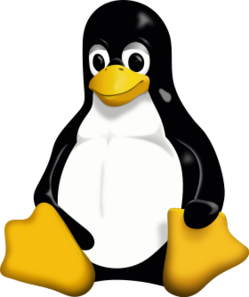
\includegraphics[width=.08\textwidth]{logo-tux.png}\hfill
  
\includegraphics[width=.3\textwidth]{logo-unab.png}\hfill
  
\includegraphics[width=.08\textwidth]{logo-python.png}
}

\makeatletter
\setbeamertemplate{title page}{
  \begin{minipage}[b][\paperheight]{\textwidth}
    \vfill%
    \ifx\inserttitle\@empty\else\usebeamertemplate*{title}\fi
    \ifx\insertsubtitle\@empty\else\usebeamertemplate*{subtitle}\fi
    \usebeamertemplate*{title separator}
    \ifx\beamer@shortauthor\@empty\else\usebeamertemplate*{author}\fi
    \ifx\insertdate\@empty\else\usebeamertemplate*{date}\fi
    \ifx\insertinstitute\@empty\else\usebeamertemplate*{institute}\fi
    \vfill
    \ifx\inserttitlegraphic\@empty\else\inserttitlegraphic\fi
    \vspace*{1cm}
  \end{minipage}
}
\makeatother


\makeatletter
\setlength{\metropolis@titleseparator@linewidth}{2pt}
\setlength{\metropolis@progressonsectionpage@linewidth}{2pt}
\setlength{\metropolis@progressinheadfoot@linewidth}{2pt}
\makeatother


\begin{document}

% ------------------------------------------------------------------------
% Portada de la Presentación
% ------------------------------------------------------------------------
\myfront{}

% ------------------------------------------------------------------------
% Slide 1: Título de la Sesión
% ------------------------------------------------------------------------
\begin{frame}
  \titlepage
  % Por ejemplo:
  % \title{Semana 9 - Sesión 2 (Sesión 18): Ejercicio Evaluado sobre POO y Datos (Semana 8) }
\end{frame}

% ------------------------------------------------------------------------
% Slide 2: Índice / Tabla de Contenidos
% ------------------------------------------------------------------------
\begin{frame}
  \frametitle{Resumen - Semana 9, Sesión 2 (Sesión 18)}
  \tableofcontents
\end{frame}

% ------------------------------------------------------------------------
% Configuración de bloques
% ------------------------------------------------------------------------
\metroset{block=fill}

% ----------------------------------------------------------------------------------------
% SECCIÓN 1: Introducción y Repaso
% ----------------------------------------------------------------------------------------
\section{Introducción y Repaso}

% ------------------------------------------------------------------------
% Slide 3: Conexión con la Semana 8 y la Sesión 9.1
% ------------------------------------------------------------------------
\begin{frame}{Repaso y Contexto}
  \begin{itemize}
    \item \textbf{Semana 8} se centró en:
      \begin{itemize}
        \item \textbf{POO básica}: clases, atributos, métodos (\_\_init\_\_).
        \item Conexión con NumPy/pandas para datos y simulaciones.
        \item Problemas evaluados en clase (sometidos a CANVAS).
      \end{itemize}
    \item \textbf{Semana 9, Sesión 1 (Sesión 17)}:
      \begin{itemize}
        \item Avanzamos en \textbf{herencia} y métodos especiales (\_\_str\_\_, \_\_repr\_\_, etc.).
        \item Ejemplos de Particle/ChargedParticle o Body/Star con distancias, potencias, etc.
      \end{itemize}
    \item \textbf{Objetivo de hoy (Sesión 18)}: Resolver un \textbf{Problema a Evaluar} que integre la POO vista en Semana 8 (clases, objetos, etc.), posiblemente con manejo de datos y breve visualización.
  \end{itemize}
\end{frame}

% ------------------------------------------------------------------------
% Slide 4: Objetivos de la Sesión 18
% ------------------------------------------------------------------------
\begin{frame}{Objetivos de la Sesión 18}
  \begin{itemize}
    \item \textbf{Consolidar} la POO aprendida en Semana 8 (clases, constructores, etc.).
    \item \textbf{Realizar} una \textbf{evaluación parcial} en grupos (25-30 minutos), subiendo el código a CANVAS.
    \item \textbf{Discutir} las soluciones y retroalimentar dudas posteriores.
    \item \textbf{Mantener} la práctica de integrar Python con NumPy/pandas, si corresponde.
  \end{itemize}
\end{frame}

% ----------------------------------------------------------------------------------------
% SECCIÓN 2: Problema a Evaluar
% ----------------------------------------------------------------------------------------
\section{Problema a Evaluar (Evaluación en Clase)}

% ------------------------------------------------------------------------
% Slide 5: Descripción del Problema
% ------------------------------------------------------------------------
\begin{frame}{Problema a Evaluar: Creación y Manejo de Clases}
  \textbf{Contexto (Semana 8):}
  \begin{itemize}
    \item Aprendimos a definir clases (POO), con \textbf{\_\_init\_\_}, métodos, atributos.
    \item Exploramos la combinación con NumPy/pandas para análisis de datos.
  \end{itemize}

  \textbf{Tareas}:
  \begin{enumerate}
    \item Definir una clase \textbf{Measurement} con atributos \texttt{name, value, unit} (por ej. “Temp”, 22.5, “C”).
      \begin{itemize}
        \item Incluir métodos \texttt{show\_info()} y \_\_str\_\_ (para impresión).
      \end{itemize}
    \item Leer (o generar) 5-10 mediciones y almacenarlas en una lista (p. ej. \texttt{measurements}).
    \item Calcular algún \textbf{estadístico} (promedio, min, max) sobre los \texttt{value} (usando NumPy, si se desea).
    \item (Opcional/Bonus) \textbf{Visualizar} con Matplotlib (barras o scatter) las mediciones, mostrando nombre vs. valor, ordenadas por valor.
  \end{enumerate}
\end{frame}

% ------------------------------------------------------------------------
% Slide 6: Instrucciones y Formato de Entrega
% ------------------------------------------------------------------------
\begin{frame}{Instrucciones para la Evaluación}
  \begin{itemize}
    \item \textbf{Equipos} de 2-3 estudiantes.
    \item Crear un \textbf{notebook} (Colab) o script local llamado \texttt{Eval\_Semana9\_Apellidos.ipynb}.
    \item \textbf{Desarrollo}:
      \begin{enumerate}
        \item Definir la clase \texttt{Measurement} (\_\_init\_\_, \_\_str\_\_, etc.).
        \item Crear 5-10 instancias manualmente o con datos generados/pedidos.
        \item Realizar un \textbf{análisis básico} de sus \texttt{value} (ej. \texttt{np.min()}, \texttt{np.max()}, \texttt{np.mean()}).
        \item (Opcional) Graficar nombres vs. valores en Matplotlib, ordenados por valor.
      \end{enumerate}
    \item \textbf{Entrega} en CANVAS antes de \textbf{25-30 min} de la clase.
  \end{itemize}
\end{frame}

% ------------------------------------------------------------------------
% Slide 7: Pautas de Evaluación
% ------------------------------------------------------------------------
\begin{frame}{Pautas de Evaluación}
  \textbf{Criterios}:
  \begin{itemize}
    \item \textbf{Funcionalidad} (40\%): ejecución sin errores, crea y maneja bien los objetos \texttt{Measurement}.
    \item \textbf{Uso de POO} (20\%): construcción de la clase, métodos, \_\_init\_\_, \_\_str\_\_ o \_\_repr\_\_.
    \item \textbf{Análisis de datos} (20\%): cálculo correcto de estadísticas (prom, min, max), uso de \textbf{NumPy} o lógicas propias.
    \item \textbf{Estilo y Organización} (20\%): comentarios, claridad, si el \textbf{opc.} gráfico se implementa con etiquetado apropiado.
  \end{itemize}
\end{frame}

% ------------------------------------------------------------------------
% Slide 8: Tiempo de Desarrollo (25-30 min)
% ------------------------------------------------------------------------
\begin{frame}{Tiempo de Desarrollo}
  \begin{block}{}
    \huge{\textbf{Tienen 25-30 minutos para resolver y subir a CANVAS.}}
  \end{block}
  \vspace{0.3cm}
  \textbf{Sugerencias}:
  \begin{itemize}
    \item Definir la clase primero, \texttt{__init__} y \texttt{__str__}.
    \item Crear una \textbf{lista} de objetos, iterar para imprimir y para extraer \texttt{values} en un \texttt{np.array}.
    \item Si grafican, consideren \texttt{plt.bar()} con \texttt{height=values} y \texttt{tick\_label=names}.
    \item Revisar antes de subir, evitando errores de sintaxis.
  \end{itemize}
\end{frame}

% ----------------------------------------------------------------------------------------
% SECCIÓN 3: Trabajo y Discusión Posterior
% ----------------------------------------------------------------------------------------
\section{Trabajo y Discusión}

% ------------------------------------------------------------------------
% Slide 9: Espacio de Resolución y Entrega
% ------------------------------------------------------------------------
\begin{frame}{Espacio de Resolución}
  \begin{itemize}
    \item Discutan en \textbf{voz baja} dentro del grupo.
    \item Preguntas puntuales a mí si se atascan (sin dar soluciones completas).
    \item Asegúrense de \textbf{ejecutar} todo antes de subir el Notebook.
  \end{itemize}
\end{frame}

% ------------------------------------------------------------------------
% Slide 10: Cierre de la Evaluación
% ------------------------------------------------------------------------
\begin{frame}{Entrega Final}
  \begin{block}{Subir a CANVAS}
    \begin{itemize}
      \item Un integrante por grupo: \textbf{notebook .ipynb} o \textbf{.py}, en el plazo establecido.
      \item Comprobar que incluya la \textbf{clase}, la \textbf{lista de objetos}, el \textbf{análisis} y, si corresponde, la \textbf{gráfica}.
      \item (Opcional) Unas líneas de explicación en Markdown.
    \end{itemize}
  \end{block}
  \vspace{0.3cm}
  \textbf{Al final}, discutiremos brevemente soluciones y dificultades encontradas.
\end{frame}

% ------------------------------------------------------------------------
% Slide 11: Discusión de Resultados
% ------------------------------------------------------------------------
\begin{frame}{Discusión Posterior}
  \begin{itemize}
    \item ¿Fue sencillo crear la \textbf{clase} y los \textbf{objetos}?
    \item ¿Cómo extrajeron \texttt{values} para el \textbf{análisis}? (Uso de NumPy vs. simple Python)
    \item ¿Quién intentó la \textbf{gráfica opcional}? ¿Qué librería usaron (\texttt{matplotlib.pyplot})?
    \item ¿El tiempo de 25-30 min fue adecuado?
  \end{itemize}
\end{frame}

% ------------------------------------------------------------------------
% Slide 12: Resumen de la Evaluación
% ------------------------------------------------------------------------
\begin{frame}{Resumen de la Evaluación}
  \begin{itemize}
    \item Integró:
      \begin{itemize}
        \item \textbf{Clases} (POO básica).
        \item Lista de objetos y algún \textbf{análisis} numérico (media, min, max).
        \item \textbf{Opción} de visualización con Matplotlib.
      \end{itemize}
    \item Apunta a \textbf{consolidar la comprensión} de POO y la manipulación elemental de datos en Python.
    \item Revisión y retroalimentación detallada se hará tras la clase.
  \end{itemize}
\end{frame}

% ----------------------------------------------------------------------------------------
% SECCIÓN 4: Cierre de la Sesión y Próximos Temas
% ----------------------------------------------------------------------------------------
\section{Cierre y Próximos Pasos}

% ------------------------------------------------------------------------
% Slide 13: Conclusiones de la Sesión 18
% ------------------------------------------------------------------------
\begin{frame}{Conclusiones de la Sesión 18}
  \begin{itemize}
    \item Realizamos un \textbf{problema evaluado} sobre POO (Semana 8) con opcional de visualización.
    \item Fortalecimos la \textbf{creación de clases} y uso de \textbf{métodos} y \textbf{atributos}.
    \item Discutimos los \textbf{resultados} y retos encontrados (tiempo, organización, sintaxis).
    \item Seguimos puliendo las bases para aplicaciones de mayor escala.
  \end{itemize}
\end{frame}

% ------------------------------------------------------------------------
% Slide 14: Próxima Sesión
% ------------------------------------------------------------------------
\begin{frame}{Próximos Temas (Semana 10)}
  \begin{itemize}
    \item Avanzar con \textbf{POO} (posiblemente herencia más compleja, polimorfismo, etc.) o nuevos módulos numéricos.
    \item Revisar \textbf{retroalimentación} de este ejercicio en la próxima clase.
    \item Si el tiempo lo permite, explorar \textbf{animaciones} en Matplotlib o \textbf{paralelización} de tareas.
  \end{itemize}
  \vspace{0.3cm}
  \textbf{Sigan practicando la POO y el manejo de datos con ejemplos propios.}
\end{frame}

% ------------------------------------------------------------------------
% Slide 15: Recursos Adicionales
% ------------------------------------------------------------------------
\begin{frame}{Recursos Adicionales}
  \begin{itemize}
    \item \href{https://docs.python.org/3/tutorial/classes.html}{\textbf{Python Docs}} - Sección de clases y POO.
    \item \href{https://numpy.org/}{\textbf{NumPy}} - para estadísticas rápidas.
    \item \href{https://matplotlib.org/stable/}{\textbf{Matplotlib}} - para visualización opcional.
    \item \href{https://canvas.instructure.com/}{\textbf{CANVAS}} - para ver feedback y calificaciones.
  \end{itemize}
\end{frame}

% ------------------------------------------------------------------------
% Slide 16: Cierre de la Sesión
% ------------------------------------------------------------------------
\begin{frame}
  \Huge{\centerline{¡Buen trabajo y nos vemos en la próxima sesión!}}
  \vspace{0.5cm}
  \normalsize
  \begin{itemize}
    \item Recuerden revisar notas/comentarios en CANVAS.
    \item ¡Sigan explorando la POO en proyectos personales!
  \end{itemize}
\end{frame}

\end{document}

